\chapter{Word Embeddings}\label{ch_word_embeddings}
\chapterauthor{Ellis Cain, Jeff Yoshimi}

% TODO: Go through chapter and add glossary items

This chapter elaborates on the concept of a word embedding, which was briefly discussed in section \extref{wrangling}. A word embedding associates each \glossary{token} in a set of tokens with a set of vectors (see chapter \extref{ch_linear_algebra}) in a way that that captures important characteristics of the set of tokens. Tokens can include words, word-parts, and other character sequences, but we focus on words here and it is standard to call these ``word embeddings'' rather than ``token embeddings'' (in fact we will often use ``word'' interchangeably with ``token'' simply as a matter of convenience).\footnote{The concept of a ``token'' varies from one context to another. Tokens can also include punctuation, emojis, or word-parts and character sequences of various kinds. Tokens are usually extracted from a corpus using automated method, for example byte pair encodings. See \url{https://en.wikipedia.org/wiki/Byte_pair_encoding}.} In this way words can be ``embedded'' in a vector space, in that a word is associated with lists of numbers that can in turn be processed by a neural network, and associated with points in a space. 

These techniques have a long history in linguistics and in the study of neural networks, but have become especially prominent in recent years with the advent of large language models (LLMs) like GPT (see chapter \extref{ch_transformers}). 
%While word embeddings may seem outdated and irrelevant due to the advent of LLMs, knowledge of the principles of word embeddings are extremely helpful for understanding LLMs due to the overlap, as these more advanced models build upon these principles and incorporate related techniques.

After giving some background on linguistics and natural language processing, we build up to the concept of a word embedding in stages. First we discuss document embeddings (associating whole documents with vectors of numbers), which are simpler to understand and serve as a useful basis for understanding word embeddings. Then we discuss word embeddings and their theoretical backing.  Then we discuss the kind of pre-processing and workflow often involved in actually taking a text and creating an embedding. Throughout the chapter, we mention connections between text embeddings\footnote{Formally a word embedding is a function from a set of tokens to a set of vectors, and a document embedding is a function from a set of documents to a set of vectors.  We will use ``text embedding'' as a generic way to cover both cases.} and neural networks, whether the neural networks are used to create text embeddings or used with text embeddings as the input.
% Finally we give a brief summary of ways neural networks are used to process linguistic data that has been numerically coded with a text embedding.\footnote{Formally a word embedding is a function from a set of tokens to a set of vectors, and a document embedding is a function from a set of documents to a set of vectors.  We will use ``text embedding'' as a generic way to cover both cases.}
Additionally, given the emphasis on converting words and other linguistic entities to vectors, this chapter overall also sheds further light on the concept of feature engineering (section \extref{wrangling}) and ``wrangling'' data so it can be used in neural networks. 

\section{Background in Computational Linguistics}

Computational linguistics is the study of language using computational methods. Analyzing large amounts of data and automating analysis for languages for under-documented language are two common applications of computational linguistics. Word embeddings originate in computational linguistics, and certain tools and concepts of the field will be useful in this chapter. 

Linguistics is the study of language, which can be organized in terms of scale, going from smallest to largest unit of study: 
\begin{enumerate}
\item Phonetics and phonology: the study of speech sounds.
\item Morphology: the study of words and word forms.
\item Syntax: the study of the structure or grammar, usually at the sentence level.
\item Semantics as the study of meaning, which can be at a variety of levels (words, phrases, sentences).
\item Pragmatics as the study of intentional meaning or implied meaning, such as implicit maxims and rules of conversations. 
\end{enumerate}

All of these levels have been studied using computational linguistics, and most of them have been studied in relation to neural networks. In some cases, features at these levels are used to generate vector representations of linguistic data (for example, word embeddings, the focus of this chapter). In other cases, neural networks have been used to analyze structures at these levels. Here is some more information on each level and their relevance to neural networks.

For spoken languages, the smallest unit would be the individual speech sounds that are used to create words. These are known as phonemes, such as the [b] in /bat/ or [p] in /pat/ and are often represented using specialized symbols of the International Phonetic Alphabet (IPA\footnote{See \url{https://en.wikipedia.org/wiki/International_Phonetic_Alphabet}}). For applications such as speech recognition or text-to-speech, researchers may need to generate representations of these sounds in vector form.  A simple way of doing this is to manually identify phonological features of phonemes and use them a binary feature vector, as in figure  \ref{elmanWordEmbeddings}, which is based on Elman's early work \cite{elman1990finding}. Phonemes can also be associated with vectors using spectrograms. A spectrogram is a plot that shows time on the x-axis, frequency on the y-axis, and uses color to indicate the intensity or amplitude at a given frequency. Converting this data into vector representation can capture the frequency content of phonemes.

\begin{figure}[h]
\centering
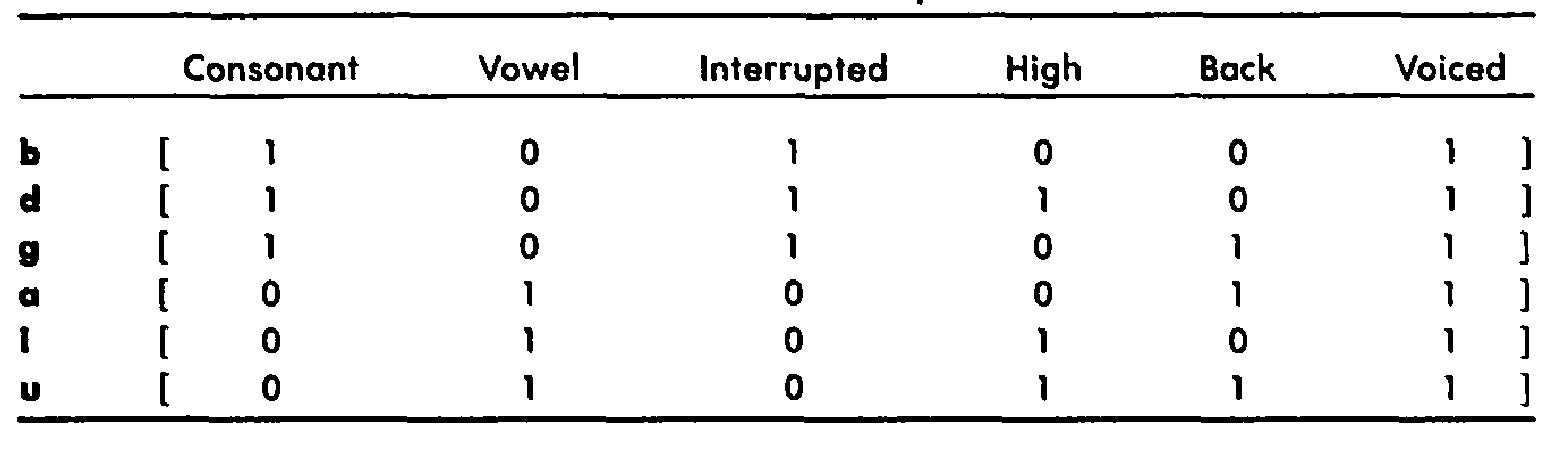
\includegraphics[scale=.5]{./images/elmanPhonemeEmbeddings.png}
\caption[From \cite{elman1990finding}.]{Some of Elman's vector representations of phonemes, which involved hand-crafted feature vectors based on linguistic attributes. This illustrates the general idea that a linguistic item (here phonemes, later tokens) can be associated with a numeric vector. }
\label{elmanWordEmbeddings}
\end{figure}

The next level up is morphology, which focuses on the smallest units of meanings at the word level (morphemes). For example, ``founded'' can be divided into two constituent morphemes ``found'' and ``-ed''.  Morphemes are used in tokenization, particularly with LLMs, such that GPT might have distinct vectors for ``found'' and ``ed''\footnote{These types of subtoken vectors assist LLMs with out-of-vocabulary issues because it allows them to recognize/represent subcomponents of an unknown word.}.  Neural networks sensitive to morphological features have played other roles historically. For example, Rumelhart and McClelland created a network that took a (phonological representation) of a verb stem as input and produced the past-tense form as output, e.g. ``look'' to ``looked'' or ``run'' to ``ran'' \cite{rumelhart1986learning}.\footnote{Given that the network must learn a regular morphological pattern (verb stem + ed) and also exceptions (e.g. run to ran), questions surrounding this model and a competing dual process symbolic model were quite prominent for a time (recall the connectionist / symbolic debate discussed in section \extref{cog_rev}). Some of the debate pertaining specifically to the past tense model is summarized in \cite{pinker2002past}.}  

Syntax studies the order and hierarchical structures of words in sentences. This includes structures such as subject-verb-object (SVO) ordering of sentences or prepositional phrase attachment (i.e., ``pet the frog [with the feather]''). Automated methods can be used to organize a representation of a sentence into grammatical categories (i.e., parts of speech) and to map out the hierarchical grammatical structure. For example, a treebank (such as the one shown in figure \ref{treeBank}, associates a sentence with part-of-speech tags that reflects syntactic or grammatical structure and dependency relationships between parts of a sentence. The question of whether neural networks can deal with grammatical structures has been at the center of the connectionist / classicist debate (again, see section \extref{cog_rev}).\footnote{Briefly, classicists have argued that grammatical structure relies on a symbolic structure that associates constituents of sentences with symbols, where those symbols can be moved around and reorganized without changing their structure. It has been argued that neural networks either fail to have this ability or if they do, simply implement a symbolic structure \cite{fodor1988connectionism}. It has also been argued that grammatical structure cannot be learned from the relatively limited stimuli available to children (``poverty of the stimulus'' arguments, \cite{berwick2011poverty}). Connectionists have responded that grammatical structure can be learned \cite{elman1996rethinking} and that they can deal with compositional structure without being mere implementations of symbol systems \cite{smolensky1988proper}.}

\begin{figure}[h]
\centering
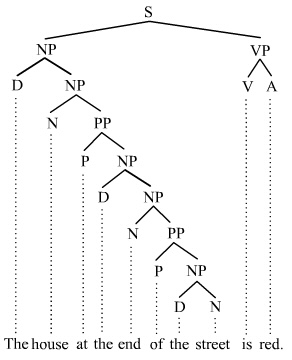
\includegraphics[scale=.45]{./images/treeBank.jpg}
\caption[From \url{https://commons.wikimedia.org/wiki/File:The_house_at_the_end_of_the_street.jpg}]{A treebank for the sentence ``The house at the end of the street'' which annotates each word with its syntactic or grammatical category and describes dependencies between parts of the sentence.}
\label{treeBank}
\end{figure}

What about the meaning of words, or semantics? Since there isn't generally a clear unit of ``meaning'' for words, this meaning level is more broad and nebulous than the others. For example, the meaning of a word can be abstract or concrete (``justice'' vs ``cup'') and is often context dependent (``bass'' as the fish or instrument). Thankfully, clever researchers have developed ways to quantify and compare meanings. One way of modeling meanings that is friendly to neural networks is using vector space or ``semantic space'' representations of word meanings, where the meaning of a word is based on its position in a network of relations \cite{erk2012vector}. Word embeddings will be the focus of this entire chapter.

The last traditional level of linguistics is pragmatics, which can be understood as the implicit rules for language use. It is often not the literal meaning of words (i.e., semantics), but rather the meaning behind the usage. For example, if you asked someone if they studied for the exam, and they said that they ``opened the textbook,'' you likely would understand that they mean that they didn't prepare well for the exam, even though their utterance does not literally mean that. Grice is well-known philosopher in this area \cite{grice1957meaning, grice1975logic}, and there has been a recent trend in using Bayesian statistics to model this type of pragmatics through Rational Speech Acts \cite{goodman2016pragmatic}. Pragmatics has not been studied much in neural networks, but has become important with LLMs since they can have actual conversations (see section \extref{ch_transformers}), and it seems likely that in modern LLMs internal representation of pragmatic structures emerge.

\section{Document embeddings}

Though our focus in this chapter will mostly be on vector representations of words, historically vector representations of whole documents are important, because they are in some cases simpler and provide a background for understanding word embeddings.

One simple approach to document embedding is the \glossary{bag of words} approach, which associates documents with vectors of word frequencies. In these representations we don't care about the order in which tokens occurs in a text, hence the term ``bag''. This approach ignores grammatical structure and just looks at how often different tokens occur in different documents. Simply put, we take each document and put the associated tokens into a bag, and count up how many tokens occur in each bag. Consider the following documents

\begin{description}
\item[Document 1]  ``The bass fish played the bass''
\item[Document 2]  ``The fish played fish with the fish monger''
\end{description}

Each document will be associated with a bag of words, as shown in figure \ref{exampleBags}.

\begin{table}[h]
    \centering
    \begin{tabular}{|l|c|c|c|c|c|c|}
    \hline
     & the & bass & fish & played & with & monger \\
    \hline
    Document 1 & 2 & 2 & 1 & 1 & 0 & 0 \\
    \hline
    Document 2 & 2 & 0 & 3 & 1 & 1 & 1 \\
    \hline
    \end{tabular}
    \caption{Bag of words representation}
    \label{exampleBags}
\end{table}

These document-level bag-of-words embeddings have a number of problems. First, they ignore the syntactic structure of the sentences in the documents they encode. Second, they are influenced by the uneven distribution of certain terms in natural languages \cite{piantadosi2014zipf, zipf1945meaning}. To counteract this, we can use term frequency-inverse document frequency (TF-IDF), a metric that measures the importance of a specific term to a (set of) related document(s). TF-IDF combines two components: term frequency (TF), which measures how often a term appears in a document, and inverse document frequency (IDF), which reduces the weight of terms that appear in many documents. These components are multiplied together, balancing the term's relevance within the document against its distinctiveness across the corpus. The ``inverse'' in IDF means that terms found in more documents receive smaller IDF values, reducing their overall influence. This ensures that TF-IDF focuses on meaningful terms rather than commonly used words like `the' or `a'.\footnote{Here is a slightly more formal definition. Consider a set of documents $D$, where for each $d \in D$ there is a set of terms $t \in d$. Then for a given term $t^*$ and document $d^*$, $\mbox{tfidf}(t^*,d^*, D) = \mbox{tf}(t^*,d^*) \cdot \mbox{idf}(t^*, D)$, where $\mbox{tf}(t^*,d^*)$ is the relative frequency of the term $t^*$ in document $d^*$ (that is, the number of times that term occurs divided by the total number of terms in the document, and $\mbox{idf}(t^*, D) = log \frac{N}{Z_{t^*}}$, where $N$ is the number of documents in $D$ and $Z_{t^*}$ is the number of times $t^*$ appears in some document in $D$. }
% Only defined for sets of documents. Places higher weight on terms that occur frequently in one document but not in others. Terms that occur frequently in all documents are given less weight (the inverse document frequency).  Does not address syntax but does deal with distribution issue. Used originally for information retrieval.  This adumbrates PPMI in word embeddings.

Latent semantic analysis (LSA) is used with a set of documents to analyze semantic information and calculate document similarity. The set of documents is represented using a document-term matrix, where each row corresponds to a document, and each column corresponds to the frequency of a given term (like bag-of-words normalized by dividing each row by the total counts in that row; try doing that for table \ref{exampleBags}). Then, singular value decomposition (SVD) is used for dimensionality reduction (on dimensionality reduction, see section \extref{S:dimred}), resulting in a numeric vector for each document (based on term usage/frequency). These vectors can then be compared using cosine similarity (section \extref{dotProduct}) to get document similarity.
% So basically SVD on bag of words
% Show a frequency table?

Researchers use these methods to calculate term frequencies in a given document or set of documents. The document embeddings can then be used to calculate document similarity, as with LSA. As we will see in the next section, these methods can also be adjusted and applied to the word level as well, allowing us to quantify word meaning as word embeddings. That is, the methods of document embeddings based on token occurrence and co-occurrence can be used to come up with word embedding techniques, and these word embeddings can be used to calculate how similar words are to each other.

\section{Word embeddings}

We now move from document embeddings to word embeddings. In this approach, instead of associating documents with vectors, we associate words or tokens with vectors. 
The general idea is that the words are embedded (or placed) into a vector space, in which the semantic information is captured and represented by the relative distance to other words in this space. Words that have similar semantic information would be near each other, and those which are unrelated would be far apart.\footnote{We describe several common approaches to word embeddings here, but there are others. For example, LLMs use a random embedding (a random association between tokens and vectors) that is trained using gradient descent. In other cases LLMs themselves are used to produce embeddings.}

Figure \ref{f:writerPainterExample} shows seven words embedded in a space. The example illustrates that the relative relations between tokens are preserved.\footnote{These were plotted using \url{http://vectors.nlpl.eu/explore/embeddings/en/}, which is a helpful interactive page for getting an intuitive feel for how word embeddings work.}  Notice that the creator of a medium (i.e., composer, author, painter) is closest to the medium or composition (i.e., music, book, painting). Interestingly, ``critic'' is closest to ``author''.

\begin{figure}[h]
    \centering
    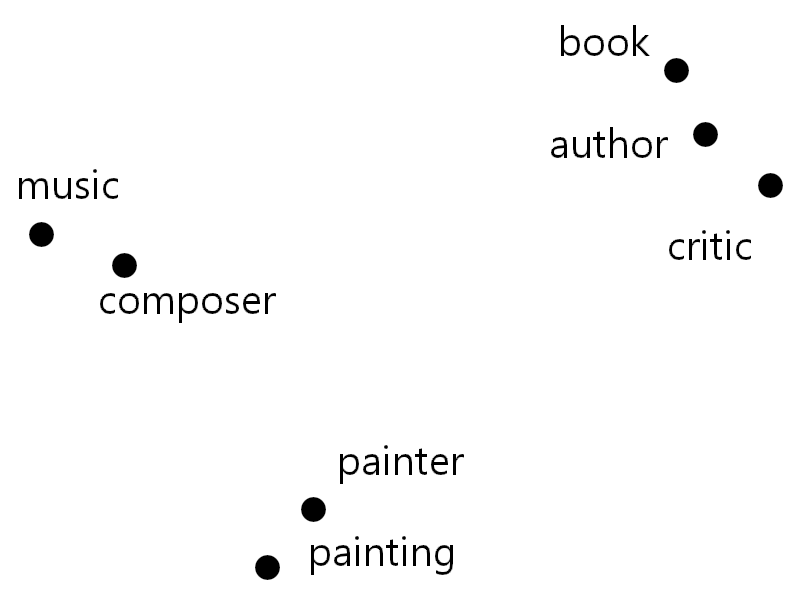
\includegraphics[scale=.2]{./images/Word_vector_demo.png}
    \caption[Adapted from an image generated using \url{http://vectors.nlpl.eu/explore/embeddings/en/}.]{Example of a word embedding in a semantic space. Each word is associated with a point in a space and the distance between points corresponds to semantic similarity. Notice that intuitively similar words are near each other in this space. }
 \label{f:writerPainterExample}
\end{figure}

Distributional semantics (DS) provides theoretical support for this approach. According to DS, information about a word's meaning is contained in linguistic context \cite{harris1954distributional, firth1957synopsis} and the statistical properties of how that word is used (i.e., a distribution of how a word is used). Distributional semantics builds on earlier usage-based theories of language such as Wittgenstein's theory of ``meaning as use'' \cite{wittgenstein1953philosophical}.\footnote{As Wittgenstein said, ``a \emph{large} class of cases of the employment of the word `meaning'... can be explained in this way: the meaning of a word is its use in the language'' (\emph{Philosophical Investigations}, section 43).} DS is often illustrated with the following quote, attributed to John Firth: ``You shall know a word by the company it keeps.'' For example, when someone talks about a \textit{river}, they may also mention \textit{water} or \textit{bank} (as in river bank), helping the listener correctly decode the intended meaning. Or, from the quote, you are able to interpret \textit{company} as referring to other words in the sentence, and not a \textit{business}, based on the earlier context.

\subsection{Co-occurrence Based Word Embeddings}

%  tracking co-occurrences allows for a rough estimation of word meaning relative to other word
% By connecting usage to meaning, this allows for an approximation or representation of meaning that is derived from usage in a text corpora. 

The high level idea with co-occurrence based embeddings is that two tokens will be close to each other in a vector space if they tend to appear near the same other words in the training corpus. Words like ``nurse'' and ``doctor'' will be near each other because they both tend to occur near words like ``hospital'', ``patient'', or ``disease''.\footnote{Thanks to Eric Schwitzgebel for this example.} In other words, because the usage of these words overlap, their meaning should be similar or related to a certain extent. 

Here is an example that illustrates the idea that words with similar meanings should be near each other in the vectors space they are embedded in (that is, they should have similar vector representations):
\begin{table}[h]
    \centering
    \begin{tabular}{|l|c|c|c|c|c|c|}
    \hline
     & Dimension 1 & Dimension 2 & Dimension 3 & Dimension 4 & ... & Dimension \textit{n} \\
    \hline
    Book    & 0.8 & 0.1 & -0.2 & 0.5 & ... & 0.7  \\
    \hline
    Critic  & 0.6 & 0.3 & -0.1 & 0.4 & ... & 0.5  \\
    \hline
    Painter & 0.2 & 0.8 & 0.4 & 0.1 & ... & -0.3 \\
    \hline
    Painting& 0.3 & 0.7 & 0.5 & 0.2 & ... & -0.2  \\
    \hline
    Music   & -0.1 & -0.4 & 0.9 & 0.3 & ... & 0.5  \\
    \hline
    Composer& -0.2 & -0.3 & 0.8 & 0.4 & ... & 0.6 \\
    \hline
    \end{tabular}
    \caption{Example of a vector space embedding in an $n$-dimensional space. The top 2, middle 2, and bottom 2 rows correspond to words that are similar and thus vectors that are near each other.}
    \label{exampleEmbeddings}
\end{table}

Note that the columns themselves (the dimensions of the vector space) don't have any clear interpretable meaning\footnote{See the linear algebra chapter. These columns are sometimes called feature but feature implies something that can be easily interpreted.}. Generally speaking, word embeddings are trained on a large text corpus (the details of how this is done using co-occurrences are given below). The resulting embeddings are often quite large, so dimensionality reduction can be used to create lower-dimensional embeddings. After dimensionality reduction, columns can no longer be interpreted as co-occurrence with specific terms in the corpus. Rather, it is the pattern across them that matters, as the relative semantic relationships between tokens are encoded in this semantic space. 

The nice thing, again, is that we can actually picture these by projecting from the high dimensional embedding space to two dimensions and then literally see the distance relationships between tokens, as in figure \ref{f:writerPainterExample}. The generated embedding space is much like our own semantic space \cite{lewis2019distributional}, with the advantage that we can track and compare word meanings mathematically and visually.

% Moved from above, since it did not fit with the context:
% Word embeddings are very important in neural networks and machine learning. 
% A widely-used word embedding is GloVe (Global Vectors for Word Representation, \cite{pennington2014glove}), which tracks the linguistic context and word co-occurrences to ``embed'' words into a semantic space. 

\subsection{Co-occurrence Matrices}

% Consider moving to end given the emphasis on practical matters.

%As we saw in the above section, instead of analyzing large corpora by hand, computational algorithms can be used to generate these numeric representations called word embeddings. 
%Here we give a high level discussion of co-occurrence based word embeddings; an actual example is worked out in section \ref{createWordEmbeddings}. Again, given that the usage of a word captures its meaning, we can track the patterns of how words occur together (i.e., co-occur), which this data is then used as the basis for word embeddings.

Based on the distributional theory mentioned above, we can track co-occurrences and usage patterns to capture the meaning of a set of words. These usages patterns are represented by a co-occurrence matrix. To construct a co-occurrence matrix, we iterate across every word in a document or training corpus and count its co-occurrences within a specified context of surrounding words. Each word is treated as a `label' or `target', while the surrounding words serve as their `context'. A window size is defined, which designates how many of the surrounding words to include in this `context'. The context can be either unidirectional, using  preceding text, or bidirectional, using surrounding context in both directions. Once the whole training corpus has been processed, the result is a co-occurrence matrix where each cell represents the raw co-occurrence counts for a given label-context pair. 

% Also good but needs to be broken out a bit more into parts and definitions.  In particular for PPMI
If, at this point, we compare across the rows of related tokens, their co-occurrences should generally be similar. Still, not every word is used with the same frequency and this may negatively impact the quality of our word embeddings. Similar to our document embeddings, some words like determiners (`the', `a') may be over-represented and skew the co-occurrence matrix. 

Generally, there are two approaches: filtering and normalization. The simplest fix is to simply filter out these high-frequency, low-impact words. These words are called  \emph{stopwords}, and various NLP packages will have stopword lists for various languages.

Another approach (usually applied in addition to removing stopwords) is to normalize word embeddings so that common words don't drown out the vector representations. A common method is using a positive-pointwise mutual information (PPMI) transform to weight the matrix.\footnote{Lenci~\cite{lenci2018distributional} explains PPMI as measuring ``how much the probability of a target-context pair estimated in the training corpus is higher than the probability we should expect if the target and the context occurred independently of one another.''} PPMI weights co-occurrence values to avoid word-frequency-bias in embeddings. Words like ``the'' and ``a'' that should not be considered meaningful in terms of co-occurrence are down-weighted. Less frequent words like ``shrubbery'' or ``herring'', that are more meaningful in terms of co-occurrences, are up-weighted. The result is a set of \textit{n}-dimensional vectors for a set of words, which are our ``word embeddings.'' For a more in-depth explanation and discussion of word embeddings and distributional semantics, see \cite{lenci2018distributional}.

\subsection{Neural Network Based Embeddings}

In addition to co-occurrence based methods, neural networks can also be used to create word embeddings. A well-known example is Word2Vec \cite{mikolov2013distributed}, which trains a simple two-weight-layer feed-forward neural network to predict targets based on the surrounding context.\footnote{A code-based walk through of the algorithm is here: \url{https://www.tensorflow.org/tutorials/word2vec}.} After the network is trained, rows from the first hidden layer weight matrix are used as the word embeddings. 
% In other words, sometimes co-occurrence based word embeddings are used as data for a neural network, whereas other times neural network based embeddings may be used for a different neural network.

% BERT, discussed in transformer chapter briefly, is also a very complex embedding, that is associated with the rise of transformers.  Used not just for word embedding but also sentence embedding. Was trained to find a masked word in a context (``masked language modeling''). What it produces is never a simple token embedding but an embedding of a word in a sentence. So it captures the meanings of words in a sentential context.  When it came out it was a new efficient way to embed a sentence. A way to get a short representation of text to summarize it, map it to images or videos etc. 

%\subsection{Trained Embeddings} % Maybe move to the transformers section?

%% Randomly intialized embeddings (they used to start with word2vec and glove but training everything end to end ends up being better.  People were surprised by that in beginning. This is what is used and has become standard to train end to end. Otherwise by initializing with certain weights you might push
% Another kind of embedding is one that is just filled with random vectors that we then train with gradient descent (see section \extref{sect_gradient_descent}) relative to some kind of task, like next word prediction (see chapter \extref{ch_transformers}), which gradually trains the embedding to work well relative to the required task. This is a surprisingly powerful method and has become a kind of de facto standard with LLMs.  The value of this kind of custom trained embedding is that the embedding ends up being well-suited to whatever task (for example next word prediction) the network is trained on.\footnote{While it may be tempting to initialize an embedding with word2vec or Glove and then train it, there is a concern that doing so might push the embedding into some region of solution space that is less optimal.}

\subsection{Geometric Properties of Word Embeddings}\label{geometryWordEmbeddings}

One striking feature of word or token embeddings is that we can perform mathematical operations on them and get semantically meaningful results. That is, the points in the embedding space that correspond to a set of tokens can be compared using addition, subtraction, and other vector operations (see chapter \extref{ch_linear_algebra}), and the results surprisingly capture how humans might conduct `operations' with concepts.  A famous paper \cite{mikolov2013linguistic} analyzed Word2Vec embeddings for hundreds of words, and found that concepts such as gender and plurality could be captured by directions in the embedding space \ref{geometryWordEmbedding}. This is the case even though the Word2Vec network was not explicitly trained to capture these concepts; it is an emergent mathematical feature of the embedding.\footnote{The way the analysis worked was that a set of analogical relationships, like ``year is to years as law is to laws'', were formulated.  For each of these relationships the last term in the analogy (here ``laws'') is searched for where the vector approach would predict it is. The word closest to this point (by cosine similarity) is identified, and can be compared with what is known to be the correct item. In this way an accuracy metric can be computed.  Accuracy scores of 62.2 \% are obtained for verbs in the original paper, and higher accuracy has been obtained in subsequent embedding models such as Glove \cite{pennington2014glove}.}

\begin{figure}[h]
\centering
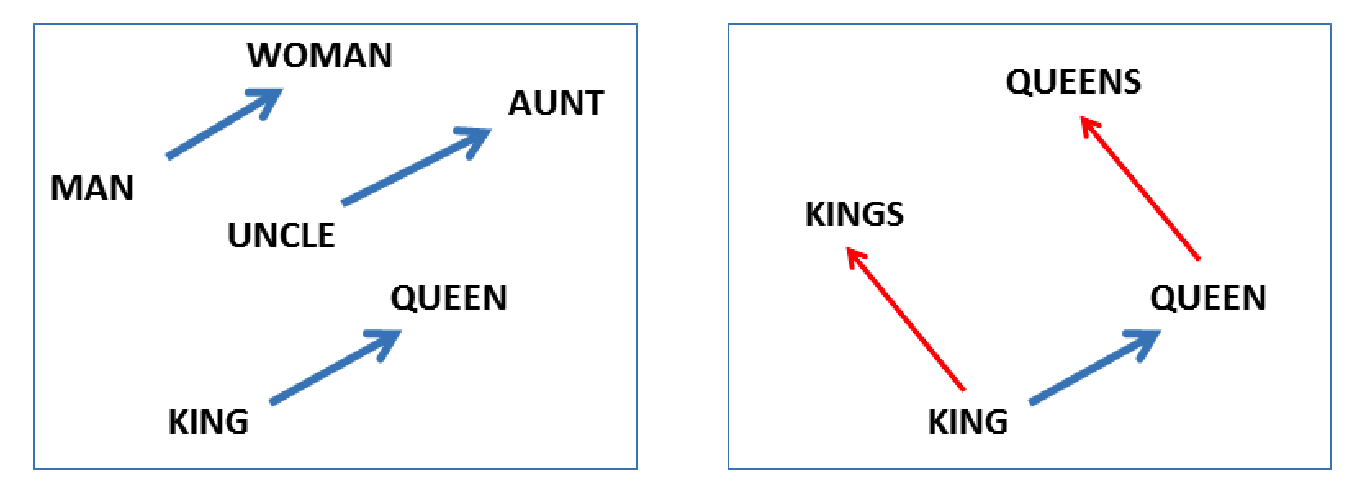
\includegraphics[scale=0.4]{./images/kingQueen.png}
\caption[From \cite{mikolov2013linguistic}.]{The left panel shows that the vectors between ``man'' and ``woman'', ``uncle'' and ``aunt'', and ``king'' and ``queen'' all point in the same direction. Thus gender appears to captured by a specific direction in the embedding space. The right panel shows a similar idea for the concept of a plural: the vectors between nouns and the plurals generally point in the same direction.}
\label{geometryWordEmbedding}
\end{figure}

In more detail, the vector difference between word embeddings that are related in similar ways are often vectors that point in the same direction (see table 1 of \cite{mikolov2013linguistic} for more examples):

\begin{itemize}
  \item $\textbf{v}_\text{apple} - \textbf{v}_\text{apples} \approx \textbf{v}_\text{car} - \textbf{v}_\text{cars}$
  \item $\textbf{v}_\text{walking} - \textbf{v}_\text{walk} \approx \textbf{v}_\text{swimming} - \textbf{v}_\text{swim}$
  \item $\textbf{v}_\text{king} - \textbf{v}_\text{queen} \approx \textbf{v}_\text{man} - \textbf{v}_\text{woman}$
  \item $\textbf{v}_\text{good} - \textbf{v}_\text{better} \approx \textbf{v}_\text{rough} - \textbf{v}_\text{rougher}$
  \item $\textbf{v}_\text{see} - \textbf{v}_\text{saw} \approx \textbf{v}_\text{return} - \textbf{v}_\text{returned}$
\end{itemize}

Using basic vector arithmetic we can derive surprising and fun relationships from those listed above which hold in the vector space, for example:

\begin{itemize}
  \item $\textbf{v}_\text{apple} - \textbf{v}_\text{apples} + \textbf{v}_\text{cars} \approx \textbf{v}_\text{car} $
  \item $\textbf{v}_\text{king} - \textbf{v}_\text{queen} + \textbf{v}_\text{woman} \approx  \textbf{v}_\text{man}$
\end{itemize}

As a reminder, these are directions in a high-dimensional space, in these models over 300 dimensions (current transformers often use embeddings with over 10,000 dimensions).\footnote{It has been shown that after about 300 dimensions the accuracy for the analogy task used in these types of analysis levels off \cite{pennington2014glove}.}  If we think of these vectors as hands on a clock, you might think we'd quickly run out of useful directions, but given that we are in high dimensional hyperspheres there are plenty of directions to go around.


\subsection{Evaluation of Word Embeddings}

% Eric pointed out this is a dense technical discussion that students could potentially skip. We can probably make that clear to students by what we assign and also just do a pass on this later

How do we know that a given word embedding accurately captures the meaning of a set of tokens? How can word embeddings be evaluated? Previous research on word similarity and relatedness has shown that directly asking for relatedness judgments can accurately capture word relations \cite{finkelstein2001placing}. Therefore, one general method of evaluation is by collecting a set of human judgements and using them to evaluate a given embedding relative (though some have questioned this approach, e.g. \cite{richie2022inter}). These can be thought of as placing a ceiling on the performance of an embedding. Several ``gold standard'' usage databases exist, such as WordSim-353 \cite{finkelstein2001placing, agirre2009study}. 

However, recent models (pre-LLM) had already reached or surpassed human performance on tasks such as similarity evaluation. Since the models have reached or surpassed theoretical performance ceilings based on human judgments, how can future improvements be evaluated? In response to this situation, Felix Hill and colleagues \cite{hill2015simlex} set out to create a standard that separates similarity from association (previous standards had ignored the distinction). Association refers to relatedness between two concepts, whereas similarity refers (almost) to synonymy. For example, ``car'' and ``tire'' would be considered associated but not similar, while ``glasses'' and ``spectacles'' are similar. While these issues are less prominent with LLMs, research remains active creating new and better benchmarks for model evaluation \cite{bugliarello2023measuring}.

Corpus quality also has an impact on model performance. Larger training corpora generally improve the quality of the derived embeddings, since the increased amount of data ideally adds more context to be processed. GloVe embeddings are trained on various training corpora, varying from 1 billion tokens to 42 billion tokens \cite{pennington2014glove}.

Besides the amount or size of the training corpora, the type of documents is also important; training solely on works of fiction would lead to different embeddings than a model trained on non-fiction, and so on.
% It is important to consider the meaning you are trying to capture (generalized or specific to a field, such as medical documents).

\section{Workflow: Creating Word Embeddings}\label{createWordEmbeddings}

In practice there are many steps involved in applying these ideas. Here is a sample workflow or pipeline:
\begin{enumerate}
\item Sentence segmentation.
\item Word tokenization
\item Normalization and filtering
\item Creation of word embeddings
\end{enumerate}

To get a sense for how this works, let's apply this pipeline to a sample document:

\begin{quote}
My work is a matter of fundamental sounds, made as fully as possible. Even though they are fundamental, they bring rich aromatic hints of humor. If people want to have headaches among the overtones, let them. And provide their own aspirin. (Adapted from a letter from Samuel Beckett to Alan Schneider, 1957)
\end{quote}

\subsection{Sentence segmentation} 

For sentence segmentation, the paragraph or document is segmented into sentences. This step is particularly important when using text that has been scanned using optical character recognition (OCR), where errors might occur. Our sample document would be segmented into four sentences (given that we are segmenting just on periods):

\begin{enumerate}
    \item \textit{My work is a matter of fundamental sounds, made as fully as possible.}
    \item \textit{Even though they are fundamental, they bring rich aromatic hints of humor.}
    \item \textit{If people want to have headaches among the overtones, let them.}
    \item \textit{And provide their own aspirin.}
\end{enumerate}

\subsection{Word tokenization} 

Once the document has been segmented into sentences, a tokenizer is used to split each sentence into the comprising words. This yields a list of lists of tokens, as in
\begin{enumerate}
    \item \textit{my, work, is, a, matter, of, fundamental, sounds, made, as, fully, as, possible}
    \item \textit{even, though, they, are, fundamental, they, bring, rich, aromatic, hints, of, humor}
    \item \textit{if, people, want, to, have, headaches, among, the, overtones, let, them}
    \item \textit{and, provide, their, own, aspirin}
\end{enumerate}

\subsection{Normalization}

Following tokenization, the words/tokens are generally normalized to remove capitalization or certain punctuation marks, such that the words are consistently in the same form. In this step, stopwords can be filtered out. In our case:
\begin{enumerate}
    \item \textit{work, matter, fundamental, sounds}
    \item \textit{fundamental, bring, rich, aromatic, hints, humor}
    \item \textit{people, headaches, overtones}
    \item \textit{provide, aspirin}
\end{enumerate}

\subsection{Create the word embeddings}

For a  basic word embedding algorithm, the label-context pair co-occurrences are tracked in a co-occurrence matrix. For the first sentence, we would start with ``work'' as the first target. Then, given a bidirectional window size of 2, the surrounding context would be ``matter'' and ``fundamental''. Therefore, the co-occurrence pairs would be [work, matter] and [work, fundamental]. We would then create a co-occurrence matrix, with targets on the rows, and context on the columns.  After processing the first sentence, the co-occurrence matrix can be seen in table \ref{exampleCoocmat}:

\begin{table}[h]
    \centering
    \begin{tabular}{|l|c|c|c|c|c|}
    \hline
    Targets & work & matter & fundamental & sounds \\
    \hline
    work & 0 & 1 & 1 & 0 \\
    \hline
    matter & 1 & 0 & 1 & 1  \\
    \hline
    fundamental & 1 & 1 & 0 & 1  \\
    \hline
    sounds & 0 & 1 & 1 & 0  \\
    \hline
    \end{tabular}
    \caption{Co-occurrence matrix. Each word vector would be a row in the matrix. Note that this is \textit{only} for the first sentence.}
    \label{exampleCoocmat}
\end{table}

Once every sentence has been processed, the final co-occurrence matrix can be seen in figure \ref{coocExample}.

\begin{figure}[h]
    \centering
    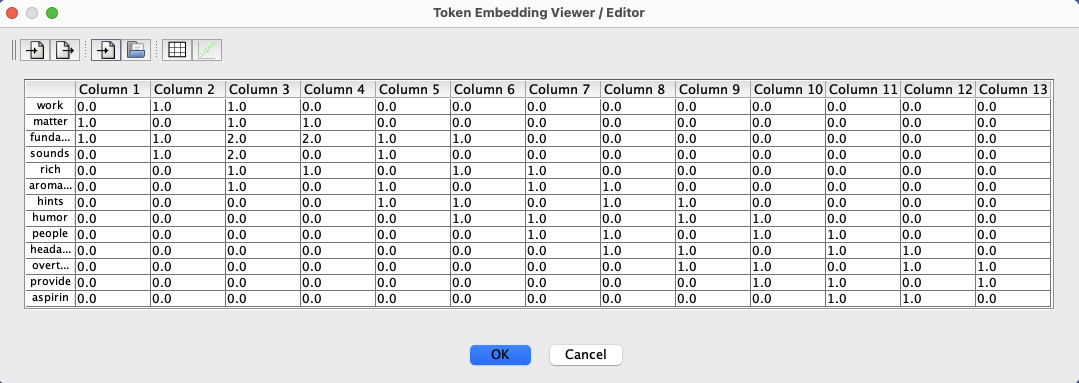
\includegraphics[scale=0.4]{./images/full_cooc_matrix.png}
    \caption[Generated using Simbrain.]{Co-occurrence matrix for the example sentences. Bidirectional window size of 2, without PPMI.}
 \label{coocExample}
\end{figure}

After processing the whole document and calculating a co-occurrence matrix, we would use PPMI to weight the vectors (recall that PPMI is used to normalize word embeddings so that common words don't drown out the representations). The result can be seen in figure \ref{ppmiExample}.

\begin{figure}[h]
    \centering
    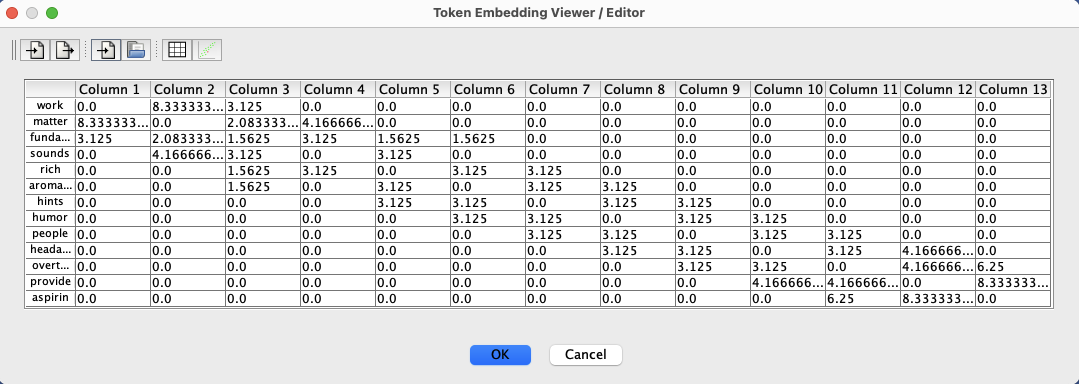
\includegraphics[scale=0.4]{./images/weighted_cooc_matrix.png}
    \caption[Generated using Simbrain.]{Resulting co-occurrence matrix after PPMI has been applied. Bidirectional window size of 2.}
 \label{ppmiExample}
\end{figure}

\subsection{Using a word embedding to make a document embedding}\label{wordEmbeddingMatrix}

Of course word embedding can be used to generate document embeddings, simply by associating each token in a document with its vector embedding and concatenating the result. Thus we can associate a whole document with a matrix, where each row is the vector embedding for one word or token in the document. A prominent example where this idea is used is with LLMs like ChatGPT (see chapter \extref{ch_transformers}), where a context window --- a set of prompts and responses --- is converted into a matrix using a vector embedding. Let's take a small, brutish context window:  ``dog chases cat and cat chases dog!''.  First we tokenize the input, then associate each token with an index, like this (notice that the punctuation mark is a token):

\begin{center}
\begin{tabular}{c@{}c@{}c@{}c@{}c@{}c@{}c@{}c}
   3 & 1 & 4 & 5 & 2 & 1 & 3 & \hspace{0.5cm}6 \\
   \texttt{dog} & \texttt{\quad chases} & \texttt{\quad cat} & \texttt{\quad and} & \texttt{\quad cat} & \texttt{\quad chases} & \texttt{\quad dog} & \texttt{\quad !} \\
\end{tabular}
\end{center}

Now we can take each integer and associate it with a row of an embedding matrix, like this, shown here with integer labels on rows to make the idea clear.
\[
\left[\begin{array}{c|ccc}
    1 & 0.5 & 0.1 & 0.3 \\
    2 & 0.2 & 0.4 & 0.6 \\
    3 & 0.7 & 0.8 & 0.9 \\
    4 & 1.0 & 1.1 & 1.2 \\
    5 & 1.3 & 1.4 & 1.5 \\
    6 & 0.3 & 0.1 & 1.2 \\
\end{array}\right]
\]

If we take each token and the corresponding row for it, and stack the results vertically, we end up with a matrix representation of a set of words (that is, a document, or in an llm, a context window), like this: 

\[
\begin{bmatrix}
    0.7 & 0.8 & 0.9 \\
    0.5 & 0.1 & 0.3 \\
    1.0 & 1.1 & 1.2 \\
    1.3 & 1.4 & 1.5 \\
    0.2 & 0.4 & 0.6 \\
    0.5 & 0.1 & 0.3 \\
    0.3 & 0.1 & 1.2 \\
\end{bmatrix}
\]

So there's our vector embedding for the document,  what we can a ``word embedding matrix'' or a ``token embedding matrix''. This matrix is suitable for processing in a neural network, like an LLM. 

You should confirm that the token embedding matrix above makes sense, that each row corresponds to the corresponding token in the sentence ``dog chases cat and cat chases dog!''